\subsection{Resultater}
Vi har kørt vores analyse på $524$ malerier, ud af vores datasæt på
$14,375$ malerier. Det svare til at $3.65 \%$ af datasættet er
gemmenløsbet. Siden vores datasæt bliver gemmenløbet alfabetisk efter
kunstnerns navn, er resultaterne, fra kunstner med efternavn startene med A
og B.


I graf \ref{antal_regioner_vertikale_cut_udvidet} er der afbilledet,
antale sammelet regioner i de 20 vertikale snit for helle datasættet.
Som man kan se er der fundet makant flere regioner i de to snit som
ligger tættest på miden, og færest ud i kanterne. 

\begin{figure}[h!]
	\begin{center}
		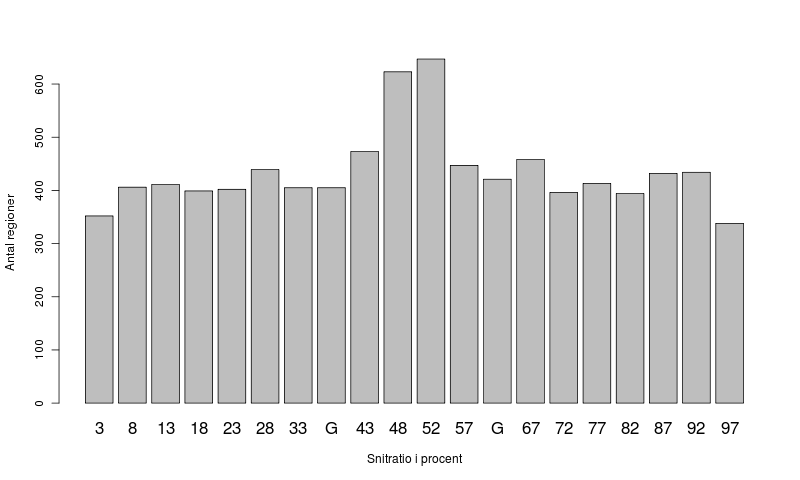
\includegraphics[width=0.9\textwidth]{afsnit/resultater/billeder/cut0cut1eatsperratioU.png}
	\end{center}
	\caption{Antal regioner i hvert af de 20 vertikale snit}
	\label{antal_regioner_vertikale_cut_udvidet}
\end{figure}

I graf \ref{antal_regioner_horisontale_cut_udvidet} er der samme
afbildning lavet, bare i det hoisontale plan, med venster side af grafen
svare til toppen af billedet. I denne graf er det 72,82 som peaker. Fra
52 og ned af, falder antal regioner gradvis. hvor i mod fra 52 og op gå
grafen lidt op og lidt ned. Kanterne er igen klart de lavest i grafen.

\begin{figure}[h!]
	\begin{center}
		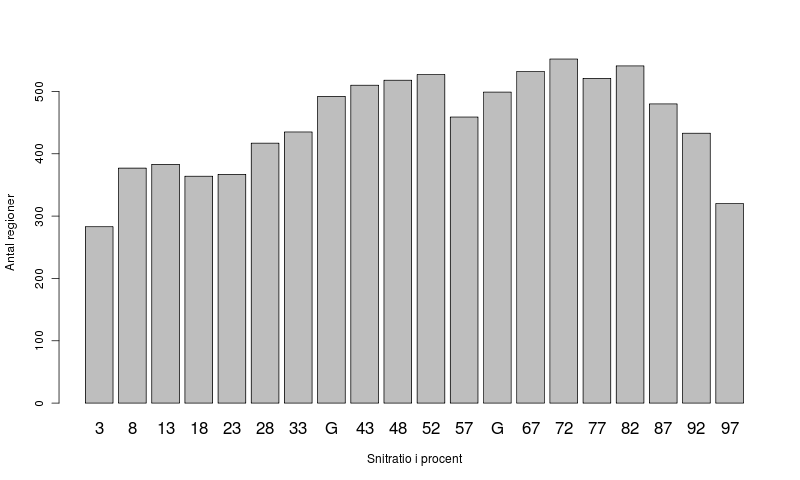
\includegraphics[width=0.9\textwidth]{afsnit/resultater/billeder/cut2cut3eatsperratioU.png}
	\end{center}
	\caption{Antal regioner i hvert af de 20 horisontale snit, hvor venstre side af grafen repræsentere øverst del af malerierne}
	\label{antal_regioner_horisontale_cut_udvidet}
\end{figure}

Ud fra disse observationer kan vi konkludere at der ikke er flere
regioner i det gyldne snit, en midden af billedet, og kan derfor
forkaste hypotese \ref{hypo_alle_andre_snit} og \ref{hypo_midten}.

I graf \ref{G_vs_to_trejedele_udvidet}, er de fire gyldne snit, samt
$\frac{2}{3}$ representeret. Som man kan se der ikke nogen entydighed på
hvad for et ration, der er dominerne, så vi kan forkaste hyptese
\ref{hypo_to_tredjedele}.

\begin{figure}[h!]
	\begin{center}
		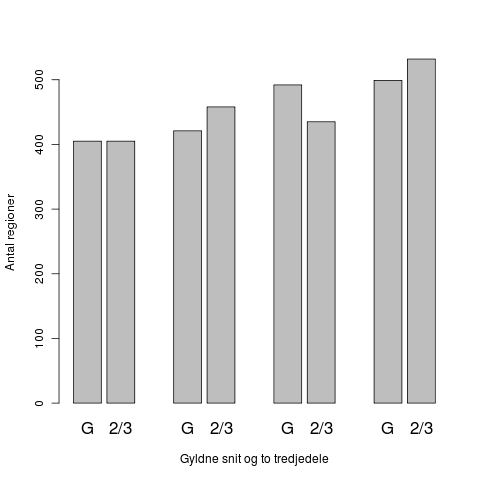
\includegraphics[width=0.6\textwidth]{afsnit/resultater/billeder/G_vs_to_tredjedeleU.png}
	\end{center}
	\caption{Procent vis antal regioner i de fire gyldne snit og deres tilhørene $\frac{2}{3}$ snit}
	\label{G_vs_to_trejedele_udvidet}
\end{figure}

\begin{table}[!h]
    \centering
    \begin{tabular}{|l|c|c|}
        \hline
            & Afvist & Ikke afvist  \\\hline
        1   &            &    \\\hline
        2   &            &    \\\hline
        3   &  			 &              \\\hline
        4   & \checkmark &              \\\hline
        5   & \checkmark &    	\\\hline
        6   & \checkmark &              \\\hline
        7   &            &              \\\hline
        8   &            &              \\\hline
        9   &            & 	\\\hline
    \end{tabular}
    \caption[]{Hypoteser i forhold til den udvidet kørsel.}
    \label{hypoteser_udvidet}
\end{table}
